In this section we just provide a graph in which we can see the evolution of the value of the contract as $S$ increases (Figure \ref{optimalPoints}). Moreover, we mark on this graph the two optimal decision points: $S_1 = 5.85$ and $S_2 = 35.58$. These two points define three regions where we would take different decisions. 

The first region is defined by $S<S_1$. Here we would sell the bond back to the issuer at $P_p=38$. In the second region, $(S_1,S_2)$, we would hold the contract. Finally, in the third region, $S_2 <\infty$, we would exercise the option and convert the bond in stock.
\vspace{-0.4cm}
\begin{figure}[h!]
	\centering
	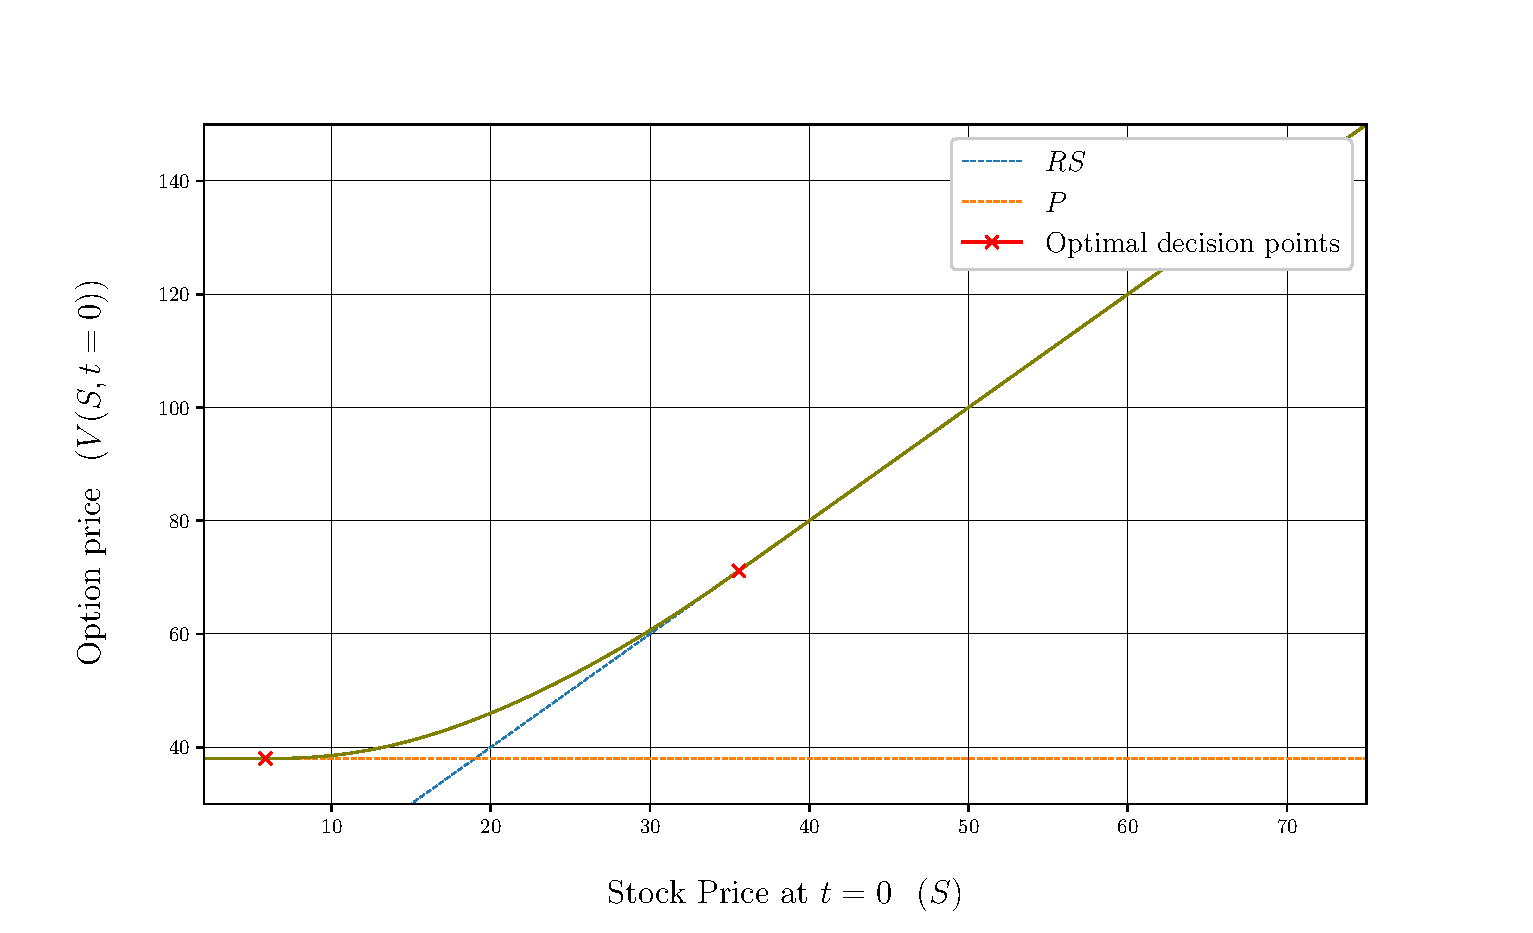
\includegraphics[scale=0.43]{img/Q2/amConvBondValues_incrS_OptimalDecisionPoints}
	\caption{Value of the contract with $r\in\{0.0058,0.0117,0.0175\}$ as $S$ increases.}\label{optimalPoints}
\end{figure}
\vspace{-0.4cm}